\documentclass[10pt]{article}

% ---- NeurIPS-like layout (built manually: the official style file could not
% be fetched here, so this approximates its look with standard packages
% rather than depending on an unverified download) ----
\usepackage[textwidth=5.5in, textheight=9in, top=1in]{geometry}
\usepackage[T1]{fontenc}
\usepackage{mathptmx}                 % Times-like text + math, NeurIPS's own choice
\usepackage{graphicx}
\usepackage{booktabs}
\usepackage{amsmath,amssymb}
\usepackage[table]{xcolor}
\usepackage{caption}
\usepackage{subcaption}
\usepackage{enumitem}
\usepackage{listings}
\usepackage[colorlinks=true, linkcolor=blue!50!black, citecolor=blue!50!black,
            urlcolor=blue!50!black, breaklinks=true]{hyperref}
\usepackage{cleveref}
\usepackage[skins,breakable]{tcolorbox}
\usepackage{titlesec}

\titleformat{\section}{\normalfont\Large\bfseries}{\thesection}{0.6em}{}
\titleformat{\subsection}{\normalfont\large\bfseries}{\thesubsection}{0.6em}{}
\titleformat{\subsubsection}{\normalfont\bfseries}{\thesubsubsection}{0.6em}{}

\lstset{
  basicstyle=\ttfamily\small,
  columns=fullflexible,
  breaklines=true,
  backgroundcolor=\color{gray!8},
  frame=single,
  rulecolor=\color{gray!40},
  framesep=4pt,
  xleftmargin=2pt, xrightmargin=2pt,
}

\newtcolorbox{findingbox}[1][]{
  colback=gray!6, colframe=black!55, boxrule=0.4pt, arc=1pt,
  left=6pt, right=6pt, top=4pt, bottom=4pt, breakable, #1
}
\newcommand{\finding}[1]{\begin{findingbox}\textbf{Finding.} #1\end{findingbox}}
\newcommand{\caveattext}[1]{\begin{findingbox}[colframe=black!30]\textbf{Caveat.} #1\end{findingbox}}
\newcommand{\status}[1]{\begin{findingbox}[colframe=black!30]\textbf{Current status.} #1\end{findingbox}}

\newcommand{\code}[1]{\texttt{#1}}

\setlength{\parindent}{0pt}
\setlength{\parskip}{0.55em}

\title{\vspace{-1.5em}\textbf{\Large System Documentation}\\[4pt]
  \normalfont\large Conversational Transfer Functions: experiment setup and
  web application, end to end}
\author{
  Kevin Kunkel \\
  \small Master's thesis, Universit\"at Leipzig \\
  \small \texttt{kevinkunkel98@gmail.com}
}
\date{\small 21 September 2026}

\begin{document}
\maketitle

\begin{center}
\begin{minipage}{0.92\textwidth}
\small
\textbf{What this document is.} \code{rl-paper.typ} argues the thesis's
claim. This document explains how the whole system is built, so that every
number, every screen, and every design decision in it can be traced to the
code that produces it. It covers the data pipeline, the transfer-function
model, the visibility measurement, the RL formulation and its four
checkpoint generations, the evaluation protocol, and the web application ---
backend, frontend, and voice --- in one place.
\end{minipage}
\end{center}

\vspace{0.5em}
\tableofcontents
\newpage

\section{System overview}

The system turns a spoken or typed instruction about a CT scan into a change
to a \emph{transfer function} --- the map from Hounsfield intensity to colour
and opacity that a volume renderer uses to decide what's visible. An
instruction like ``show only the lungs'' or ``a bit less soft tissue'' is
parsed into a structured command, turned into a \emph{goal} (a target change
in how visible and how bright each anatomical class should be), and answered
one of three ways: applied directly by a fixed rule, hill-climbed by search,
or proposed in one forward pass by a trained reinforcement-learning policy.

\begin{figure}[h]
  \centering
  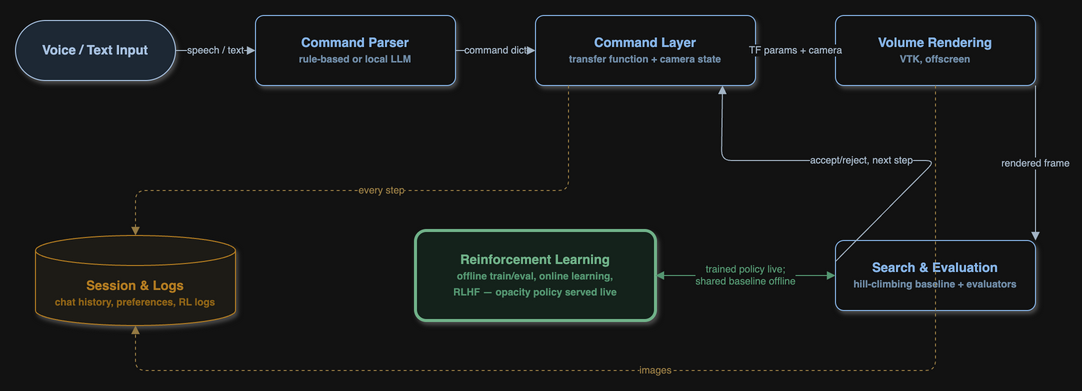
\includegraphics[width=0.92\linewidth]{screenshots/architecture-highlevel-dark.png}
  \caption{High-level data flow. Voice or text reaches the command parser;
  the parsed command becomes transfer-function parameters and camera state;
  volume rendering (VTK) and the cheap visibility estimate both consume those
  parameters; every step is logged to the session. Search/evaluation and RL
  sit beside the command layer, not inside the request path, except when the
  \textbf{search} or \textbf{policy} answer mode is explicitly chosen.}
  \label{fig:architecture}
\end{figure}

\caveattext{This diagram predates today's session and is a simplification in
two respects worth knowing before reading it literally: ``RLHF'' and
``trained policy live'' describe the \emph{intended} end state, not the
current one --- see \cref{sec:preferences} for the actual status (0 clean
preference judgments, reward model not yet trained). And the one-shot policy
(\cref{sec:rl-formulation}) answers in a single forward pass, not through the
iterative accept/reject loop the arrows towards ``Search \& Evaluation''
suggest; that loop describes the hill-climb baselines specifically.}

\subsection{Component map}

\begin{table}[h]
\centering\small
\begin{tabular}{@{}ll@{}}
\toprule
\textbf{Module} & \textbf{Responsibility} \\
\midrule
\code{server.py} & FastAPI backend: session state, rendering, every API route \\
\code{static/} & Frontend: \code{index.html}, \code{app.js}, \code{viewer.js}, \code{style.css} \\
\code{commands.py} & Instruction grammar: rule parser, LLM parser, \code{apply\_command} \\
\code{asr.py} & Voice transcription (faster-whisper) \\
\code{transfer.py} & The 24-parameter transfer-function model and its VTK/opacity math \\
\code{render.py}, \code{views.py} & Offscreen VTK rendering, the six standard camera views \\
\code{visibility.py} & Cheap per-class visibility/brightness estimate, validated against VTK \\
\code{goals.py} & Instructions $\rightarrow$ goal vectors; the distance/attainment objective \\
\code{rl/} & Environments, training, baselines, evaluation \\
\code{datasets.py}, \code{totalseg.py} & Volume loading, splits, anatomical labels \\
\code{collect.py} & Blind pairwise preference collection for RLHF \\
\code{tools/} & Data selection, cache building, validation, reports \\
\code{plots/} & Figure generation from \code{rl.vis\_eval} result files \\
\bottomrule
\end{tabular}
\caption{Every module referenced in this document, and where to find it.}
\end{table}

\newpage
\section{Data pipeline}

30 CT scans from the TotalSegmentator ``small'' subset (CC-BY-4.0),
stratified by body region into 20 training, 4 validation, and 6 test
subjects, plus four 3D Slicer sample CTs (\code{ct\_chest}, \code{ct\_skull},
\code{ct\_cardio}, \code{ct\_abdomen}) held out as an \emph{out-of-source}
generalisation set from different scanners.

\begin{lstlisting}
curl -L -o data/Totalsegmentator_dataset_small_v201.zip \
  "https://zenodo.org/records/10047263/files/Totalsegmentator_dataset_small_v201.zip?download=1"
python -m tools.select_totalseg          # select, label, split -> data/totalseg_manifest.json
python -m tools.build_visibility_cache   # precompute visibility caches
\end{lstlisting}

Selection is deterministic and committed as \code{data/totalseg\_manifest.json},
so the splits reproduce without redistributing the scans themselves. Each
manifest entry records the subject id, split, SHA-256, whether it's a
contrast-enhanced scan, and which of the five measured anatomical classes are
present in its segmentation. Volumes load in canonical RAS orientation
(\code{totalseg.load\_volume}); \code{python -m tools.check\_orientation
<name>} writes projection images to verify it by eye.

\begin{table}[h]
\centering\small
\begin{tabular}{@{}lccl@{}}
\toprule
\textbf{Split} & \textbf{Subjects} & \textbf{Contrast} & \textbf{Notes} \\
\midrule
train & 20 & 3 & drives both RL training and instruction sampling \\
val & 4 & 1 & checkpoint selection during training, by median attainment \\
test & 6 & 1 & held out; every number in \cref{sec:results} comes from here \\
out-of-source & 4 (Slicer) & 1 (\code{ct\_cardio}) & never trained on; not formally evaluated, \cref{sec:limitations} \\
\bottomrule
\end{tabular}
\caption{The manifest's split sizes. ``Contrast'' counts subjects with
\code{contrast: true}, the gate that makes \code{vessels} a measurable goal
(\cref{sec:vessels-gate}) --- only 5 of 30 TotalSegmentator subjects qualify,
and only one of the six test subjects (\code{ts\_s1379}).}
\end{table}

\caveattext{The out-of-source Slicer CTs have no TotalSegmentator labels at
all. \code{visibility.py} falls back to a coarse intensity-band classifier
for them (\cref{sec:intensity-fallback}), and the policy has never seen them
during training. A live check found the policy performing at or below ``do
nothing'' on \code{ct\_skull}; see \cref{sec:limitations}.}

\newpage
\section{The transfer-function model}
\label{sec:tf-model}

A transfer function is 24 floating-point numbers: four peaks, six values
each, every value normalised to $[-1, 1]$.

\begin{table}[h]
\centering\small
\begin{tabular}{@{}ll@{}}
\toprule
\textbf{Index (within a peak)} & \textbf{Meaning} \\
\midrule
0 & centre, mapped to Hounsfield units over \code{CENTER\_RANGE} $= (-1050, 2000)$ \\
1 & width in HU, mapped over \code{WIDTH\_RANGE} $= (10, 400)$ \\
2 & height (opacity), unit interval \\
3--5 & colour, RGB, each a unit interval \\
\bottomrule
\end{tabular}
\caption{\code{transfer.PARAMS\_PER\_PEAK = 6}. A peak's opacity at a
Hounsfield value $h$ is a Gaussian: $\text{height} \cdot
\exp\!\big(-0.5\,((h-\text{centre})/\text{width})^2\big)$, summed and clipped
to $[0,1]$ across all four peaks; colour is the opacity-weighted blend of
each peak's own colour.}
\end{table}

The \emph{anatomical layout} (\code{transfer.anatomical\_params}, what every
session and every training episode starts from) places one peak per goal
class, centres fixed for the life of the system --- no command and no policy
action ever moves a centre:

\begin{table}[h]
\centering\small
\begin{tabular}{@{}lcccc@{}}
\toprule
\textbf{Class} & \textbf{Peak index} & \textbf{Centre (HU)} & \textbf{Width (HU)} & \textbf{Default height} \\
\midrule
lungs & 0 & $-800$ & 60 & 0.05 \\
soft tissue & 1 & 40 & 80 & 0.15 \\
vessels & 2 & 300 & 80 & 0.30 \\
skeleton & 3 & 900 & 280 & 0.60 \\
\bottomrule
\end{tabular}
\caption{\code{transfer.ANATOMICAL\_*} constants. A command or the policy can
change a peak's height, width, or colour; it can never move its centre or
reassign which class a peak represents.}
\label{tab:anatomical}
\end{table}

\finding{Skeleton's width (280 HU) is far wider than the others. Boosting its
height still puts real opacity into a neighbour's HU range --- this is
precisely the mechanism behind the ``show only'' haze fixed in
\cref{sec:show-only-width}, and it is also the reason the \emph{original}
pre-RL-v2 version of this project failed (\cref{sec:evolution}): ``more
bone, less spongy'' required narrowing the bone peak, and the system had no
way to ask for that.}

An earlier, retired layout (\code{transfer.default\_params}, before a fix on
2026-09-16) placed peak 0 at fat ($-100$ HU) rather than lung parenchyma. It
now simply returns \code{anatomical\_params()}; the distinction is kept in
this document only because older screenshots and one retired docstring still
describe the band layout.

\newpage
\section{Measuring what a render shows}
\label{sec:measure}

Direct volume rendering is too expensive to run inside a search loop or an
RL step (50--210\,ms), and a rendered image alone doesn't say \emph{which
tissue} produced which pixel. \code{visibility.py} estimates both cheaply:

\begin{enumerate}[itemsep=2pt, topsep=2pt]
\item Resample the volume once per viewing direction into an $80^3$ cube
  (\code{GRID\_N}) whose first axis runs front to back
  (\code{VisibilityModel.from\_volume}).
\item Resample the anatomical label volume the same way (nearest-neighbour,
  not interpolated --- interpolating across a tissue boundary would invent a
  label the volume doesn't actually contain there).
\item For a given transfer function, composite front to back: weight $=
  \alpha \cdot \prod(1-\alpha_{\text{before}})$, using an opacity/colour
  lookup table quantised to 256 levels over the same HU range the transfer
  function is defined on.
\item Sum each class's weight and divide by the ray count for that class's
  \code{vis} (share of the final image it contributes); the weight-averaged
  colour luminance is \code{bright}; the fraction of rays whose accumulated
  opacity clears 0.3 is \code{coverage}.
\end{enumerate}

This runs in about 14\,ms on CPU, six standard views per volume (\code{views.N\_VIEWS}).

\subsection{Validation against real renders}
\label{sec:validation}

The reference renders the same transfer function twice --- once normally,
once with one class's \emph{colour} blacked out and its \emph{opacity}
untouched, via VTK label-map masking --- and takes the difference in mean
luminance as that class's true contribution.

\finding{Deleting a class's voxels instead --- the obvious first method ---
measures something else, because the hole left behind reveals whatever sits
behind it. On a bone-dominant transfer function: 0.1481 normally, 0.1065 with
skeleton's colour blacked out (its true contribution), 0.1194 with
skeleton's voxels \emph{deleted} --- higher, because the background showed
through. Thin surface tissue anti-correlated with its own visibility under
the deletion method.}

\begin{table}[h]
\centering\small
\begin{tabular}{@{}lccccl@{}}
\toprule
\textbf{Class} & \code{ts\_s1379} & \code{ts\_s1337} & \code{ts\_s0454} & \textbf{Status} & \textbf{Notes} \\
\midrule
skeleton & 1.000 & 0.999 & 1.000 & validated & \\
organs & 0.995 & 0.994 & 0.969 & validated & \\
muscle & 0.981 & 0.948 & 0.999 & validated & \\
vessels & 0.992 & 0.989 & (0.001 range) & validated & contrast scans only \\
lungs & 0.89--0.97 & --- & --- & validated & corrected, see below \\
\bottomrule
\end{tabular}
\caption{Pearson correlation between the estimate (visibility $\times$
brightness) and the label-masked render reference, 10 transfer functions per
class, over the volumes checked.}
\end{table}

\caveattext{Lungs were previously reported here as unvalidated ---
``below the renderer's noise floor'' --- and that was wrong. The
reachable-ceiling probe (\code{solo\_max}) that decides whether a class's
contribution is measurable at all was built from the \emph{retired} band
layout, whose first peak sits at fat ($-100$ HU), nowhere near lung
parenchyma ($-800$ HU). Measured through the correct peak, lungs validate
like any other class on five of six checked volumes.}

\subsection{The ``other'' bucket}
\label{sec:other-bucket}

As of today, \code{features()} also reports \code{vis["other"]}: the share of
the image contributed by voxels the label volume (or the intensity fallback)
assigns to \emph{none} of the five classes --- fat, connective tissue,
partial-volume edges. This did not exist before this session; see
\cref{sec:v4-fix} for why it was added and what broke without it.

\subsection{The intensity fallback}
\label{sec:intensity-fallback}

Any volume that isn't a \code{ts\_*} TotalSegmentator subject (the four
out-of-source Slicer CTs, the synthetic phantom) has no anatomical labels at
all. \code{visibility.\_intensity\_class\_ids} falls back to coarse
Hounsfield bands: $\le -500$\,HU is lungs, $-30$ to $300$\,HU is organs,
$\ge 300$\,HU is skeleton. Muscle and vessels are never populated by this
fallback --- there is no contrast information to separate them from soft
tissue or bone --- so \code{goals.FALLBACK\_GOAL\_CLASSES} excludes vessels
on every volume that isn't a contrast-flagged TotalSegmentator subject.

\newpage
\section{Instructions, goals, and scoring}

\subsection{From words to a command}

Two parsers turn free text into the same structured command shape
(\code{\{"target", "attribute", "direction", "strength"\}}, or a
\code{"compound"} list of these):

\begin{itemize}[itemsep=2pt, topsep=2pt]
\item \textbf{Rule parser} (\code{commands.parse\_command\_rule}): a fixed
  set of regexes over a vocabulary of class synonyms (\code{CLASS\_SYNONYMS})
  and verbs (\code{DIRECT\_VERBS} --- sharpen/soften/brighten/darken/hide/remove).
  Deterministic, no external dependency, and the ground truth
  \code{rl.baselines.current\_executor} mirrors.
\item \textbf{LLM parser} (\code{commands.parse\_command\_llm}): a local
  Ollama model (\code{qwen2.5:7b} by default) given a system prompt
  describing the exact JSON schema, with a 30\,s timeout. Falls back to the
  rule parser automatically --- on a connection error, an invalid schema, or
  a missing target --- so a live demo never hard-fails on an LLM hiccup.
\end{itemize}

\status{The viewer's own default (\code{static/app.js}, and \code{server.py}'s
\code{CommandRequest}/\code{CompareRequest} defaults) is \code{"llm"}, not
\code{"rule"} --- voice input benefits most from the LLM's tolerance for
varied phrasing. Internal callers that need determinism (the RL
training/eval pipeline, and most of the test suite) explicitly request
\code{"rule"} instead of relying on a default.}

A parsed command becomes a \emph{goal} (\code{goals.goal\_from\_command}):
for each named class, a requested change in $\log_{10}$ visibility and/or
brightness. ``Show only'' is special-cased (\code{\_goal\_show\_only}): named
classes get $+1.0$ ($10\times$ more visible, \code{HIDE\_STRENGTH}), every
other measurable class gets $-1.0$.

\subsection{The objective}
\label{sec:objective}

\begin{equation*}
\begin{aligned}
D = \; & \sum_i m_i |c_i - d_i| \;+\; \kappa \sum_i n_i |b_i - e_i| \\
       & + \lambda \sum_i (1-m_i) \max(0, |c_i| - \tau) \;+\; \lambda \kappa \sum_i (1-n_i) \max(0, |b_i| - \tau) \\
       & + \lambda \max(0, |c_{\text{other}}| - \tau)
\end{aligned}
\end{equation*}

with $\kappa = 1.5$ (\code{KAPPA}), $\lambda = 0.3$ (\code{LAMBDA\_KEEP}),
$\tau = 0.15$ (\code{KEEP\_TOLERANCE}); $c_i$, $b_i$ are the achieved
$\log_{10}$-visibility and brightness changes relative to the episode's
start state, $d_i$/$e_i$ the requested changes, $m_i$/$n_i$ whether class
$i$'s visibility/brightness was named at all. \emph{Attainment} is reported
throughout: $A = 1 - D_{\text{final}}/D_{\text{start}}$, so 1 means the goal
was reached, 0 means no better than doing nothing, negative means worse.

\finding{The keep-tolerance $\tau$ is load-bearing, and so --- as of today
--- is its extension to unclassified tissue. Moving one peak always disturbs
something adjacent a little, even when the instruction is followed well; a
keep term that punished \emph{any} drift, or one that ignored unclassified
tissue entirely, would each make leaving the transfer function untouched
score better than acting on the instruction. See \cref{sec:v4-fix} for the
concrete failure this closed.}

\subsection{Instruction kinds and sampling}
\label{sec:instruction-mix}

Both training episodes and the held-out evaluation draw from the same
grammar (\code{goals.sample\_instruction}, \code{goals.INSTRUCTION\_MIX}):

\begin{table}[h]
\centering\small
\begin{tabular}{@{}lcl@{}}
\toprule
\textbf{Kind} & \textbf{Share} & \textbf{Example} \\
\midrule
relative & 40\% & ``a bit less soft tissue'' \\
compound & 25\% & ``more bone, a bit less soft tissue'' \\
show only & 15\% & ``show only the lungs and skeleton'' \\
absolute & 10\% & ``high opacity vessels'' \\
brightness & 10\% & ``brighten the skeleton'' \\
\bottomrule
\end{tabular}
\caption{The sampled instruction mix every episode (training, validation,
and the 200-episode held-out test) is drawn from.}
\end{table}

A goal class is only sampled when it's reachable at all:
\code{VISIBLE\_CEILING = 0.005} --- below half a percent of the image under
the best single-peak transfer function, a change is measurable but not
something a person could judge, so it's excluded from sampling entirely
(this is what silently refuses lung instructions on four of six test
subjects, and vessel instructions on all but one).

\subsection{\code{vessels} requires contrast}
\label{sec:vessels-gate}

\code{goals.goal\_classes\_for\_volume} only offers \code{vessels} as a goal
when the volume is a \code{ts\_*} TotalSegmentator subject \emph{and} its
manifest entry has \code{contrast: true} \emph{and} \code{"vessels"} appears
in its segmentation. None of the picker's six friendly-named demo datasets
(\code{ct\_chest}, \code{ct\_skull}, \code{ct\_cardio}, \code{ct\_abdomen},
\code{mri\_head}, \code{stag\_beetle}) satisfy this --- \code{ct\_cardio}
included, despite its name --- because none of them are TotalSegmentator
subjects at all. In the running viewer, vessels is answerable on exactly one
dataset: \code{ts\_s1379}.

\newpage
\section{The reinforcement-learning formulation}
\label{sec:rl-formulation}

\subsection{Why one-shot, not ten steps}

The first formulation gave the policy ten steps of $\pm 0.1$ per parameter,
rewarding the drop in goal distance at each step. It never learned, and
training longer made it \emph{worse} --- flat to degrading across every
setting tried (reward scale, exploration, gradient steps per env step).

\finding{The diagnosis is structural. A ten-step policy must commit to each
change \emph{blind}; the hill-climber it's measured against may try a
change, measure it, and reject it. It was being asked to learn a search
procedure --- a strictly harder problem than the mapping the thesis actually
asks about, and one a 10-evaluation search already does well. Emitting the
whole transfer function in one forward pass removes the search from the
policy's job and leaves only the mapping.}

\subsection{Observation, action, reward}

\code{rl.oneshot\_env.OneShotEnv}, one step per episode:

\begin{table}[h]
\centering\small
\begin{tabular}{@{}p{2.6cm}p{10.5cm}@{}}
\toprule
\textbf{Component} & \textbf{Definition} \\
\midrule
Observation (57) & goal vector (16) + intensity histogram (16) + per-class
$\log_{10}$ visibility (4) + brightness (4) + $\log_{10}$ reachable ceiling
(4, \code{solo\_max}) + current controllable parameters (12) + coverage (1) \\
Action (12) & the new \emph{value} --- not a delta --- of each controllable
group: height, width, and colour per peak, in $[-1,1]$; centres are never
controllable \\
Reward & \code{attainment}, clipped to $[-1,1]$, minus 1.0 if the result
shows effectively nothing (\code{goals.is\_useless}: coverage $<1\%$ or total
visibility $<0.1\%$) \\
Episode & exactly one step \\
\bottomrule
\end{tabular}
\caption{The one-shot environment every checkpoint from v1 onward trains against.}
\end{table}

Reset noise: each controllable group gets uniform $\pm 0.3$ noise
(\code{START\_NOISE}) added to the anatomical default before the episode
starts, so the policy sees more than one exact starting point per volume.

\subsection{Hindsight relabelling --- implemented, not used}

\code{OneShotEnv} supports \code{hindsight\_ratio}: with that probability, an
episode draws a \emph{reachable} random action first, measures what it
achieved, and uses that as the goal instead of a sampled instruction ---
guaranteeing every such episode has a demonstrated solution. The noise scale
(0.25 controllable units) is calibrated against 200 synthetic episodes to
land in the same delta range real instructions ask for.

\caveattext{\code{hindsight\_ratio} defaults to \code{0.0}, and the actual
training invocation used for every checkpoint in \cref{sec:evolution} does
not override it. This machinery is fully built and calibrated but has never
been turned on in a run that produced a reported number.}

\subsection{Training}

\begin{lstlisting}
python -m rl.oneshot_train --timesteps 150000 --seed {0,1,2} \
  --eval-interval 10000 --out out/rl_v2/oneshot_v{N}_seed{seed}
\end{lstlisting}

SAC (\code{stable\_baselines3.SAC}, \code{MlpPolicy}), one override from
library defaults: \code{learning\_starts=500} (vs.\ 100), giving the replay
buffer a few more random episodes before learning starts. Every
\code{eval-interval} steps: 40 fixed validation episodes, deterministic
action, logged to \code{eval\_progress.csv}; the checkpoint is kept as
\code{best.zip} by \emph{median} attainment, not mean --- a single
very-negative episode on an easy goal (attainment is unbounded below) can
otherwise swing which checkpoint looks best.

\subsection{Baselines}

\begin{table}[h]
\centering\small
\begin{tabular}{@{}lp{9.3cm}c@{}}
\toprule
\textbf{Baseline} & \textbf{Mechanism} & \textbf{Evals} \\
\midrule
B0 do nothing & returns the start state unchanged & 0 \\
B1 rule executor & named class(es) to height 0.7 (width capped to 150\,HU
  as of today for \code{show\_only}, \cref{sec:show-only-width}), one
  asymptotic step per mentioned class otherwise & 0 \\
B2 random & 10 random $\pm 0.1$ steps, ignoring the instruction entirely --- the floor & 0 \\
B3/B4 hill-climb & coordinate search directly minimising the objective
  (\cref{sec:objective}): try $\pm$step on each of 12 dims, keep
  improvements, halve the step when a sweep finds none & 10 / 200 \\
B5 occlusion rule & B1, then crushes every peak not named or increasing to height 0.02 & 0 \\
\bottomrule
\end{tabular}
\caption{Every baseline \code{rl.baselines} implements. B3/B4 have
\emph{oracle access} to the exact scoring function at inference time; the
policy and B0/B1/B2/B5 never see \code{goals.distance} outside training.}
\end{table}

\newpage
\section{Evolution of the policy: v1 through v4}
\label{sec:evolution}

The one-shot formulation went through four checkpoint generations. Each was
retrained from scratch, not fine-tuned from the previous one, so a later
generation's numbers never carry an earlier bug's habits forward.

\begin{table}[h]
\centering\small
\begin{tabular}{@{}lp{2.6cm}p{8.7cm}@{}}
\toprule
\textbf{Version} & \textbf{Checkpoints} & \textbf{What changed} \\
\midrule
v1 & \code{oneshot\_seed\{0,1\}} & First one-shot checkpoint, replacing the
  ten-step formulation. No held-out evaluation was ever run against it ---
  superseded within a day by v2. A 53-value observation (no
  reachable-ceiling channel). \\
v2 & \code{oneshot\_v2\_seed\{0,1,2\}} & Added the reachable-ceiling channel
  to the observation (57 values). Evaluated, but on two undetected bugs, below. \\
v3 & \code{oneshot\_v3\_seed\{0,1,2\}} & Both bugs fixed. Headline checkpoint
  from 2026-09-17 until today. \\
v4 & \code{oneshot\_v4\_seed\{0,1,2\}} & \code{goals.distance} gained the
  ``other'' keep term (\cref{sec:v4-fix}) --- a gap v1 through v3 all shared.
  \emph{Current}, shipped in the viewer as seed 2. \\
\bottomrule
\end{tabular}
\caption{Directory names under \code{out/rl\_v2/} match this table's version
column exactly.}
\end{table}

\subsection{v2's two bugs, and what fixing them was worth}

v2's reachable-ceiling probe (\code{solo\_max}) was built from
\code{default\_params()} --- the retired band layout --- so peak 0 was
probed as fat, not lungs, the same mismeasurement described in
\cref{sec:validation}. Separately, \code{CONTROLLABLE} groups a peak's
$(r,g,b)$ into one value (its mean); the one-shot policy \emph{set} that
group instead of adding a delta to it, which wrote the same scalar into all
three channels --- every policy render came out grey, while every baseline
stayed coloured, so a rater could tell which candidate was the policy's on
sight. Six preference judgments collected under this bug are archived
(\code{out/vis\_preferences\_pre\_colour\_fix.jsonl}) rather than used.

\begin{table}[h]
\centering\small
\begin{tabular}{@{}lccc@{}}
\toprule
\textbf{Statistic} & \textbf{v2} & \textbf{v3} & \textbf{Gap} \\
\midrule
median of seed medians & $+0.247$ & $+0.275$ & $+0.028$ \\
median of seed-averaged per-episode & $+0.201$ & $+0.286$ & $+0.086$ \\
\bottomrule
\end{tabular}
\caption{Same 200 episodes, two aggregations. Paired Wilcoxon on the
seed-averaged per-episode values: $p = 0.0064$, v3 ahead on 59\% of episodes.
The gain concentrates in \emph{absolute} instructions ($+0.122$ of $+0.038$
average kind-level gain) --- exactly the kind whose target is a share of the
reachable ceiling, the channel that was repaired.}
\end{table}

\caveattext{A published intermediate figure ($+0.169$ for v3) was a
measurement accident, not a defect in the policy: the evaluation job was
started before the ceiling fix landed and finished six hours after, so it
scored with the code the process had loaded at import time, not the code on
disk. \code{provenance.py} now records the git commit and a fingerprint of
the imported scoring modules in every result file specifically so this
can't recur silently.}

\subsection{v3 to v4: fixing a reward-hacking blind spot}
\label{sec:v4-fix}

\code{visibility.py} measured five classes, but every voxel belonging to
none of them was invisible to the objective --- not measured, not
penalised, not present anywhere in \code{goals.distance}.

\finding{A transfer function could satisfy ``show only X'' by rendering an
opaque wall of unclassified tissue instead of X. Driving \code{hill\_climb}
(200 evaluations) on ``show only bones'' reached \emph{full frame coverage}
while every one of the five labelled classes read below 0.001 of the image
--- 99\% of the frame was material the objective could not see, and the
search still scored it as a strong answer, because nothing charged for it.}

Fix: \code{visibility.py}'s \code{features()} gained an \code{"other"}
bucket (\cref{sec:other-bucket}); \code{goals.distance} charges for it under
the same keep-tolerance any unmentioned class already gets
(\cref{sec:objective}). Verified in isolation before retraining --- new unit
tests confirm a transfer function that hides a class behind unclassified
material now scores strictly worse than hiding it cleanly.

\begin{table}[h]
\centering\small
\begin{tabular}{@{}lccc@{}}
\toprule
\textbf{Method} & \textbf{v3} & \textbf{v4} & \textbf{Improved} \\
\midrule
hill-climb (thorough) & $+0.730$ & $+0.692$ & $100\% \rightarrow 100\%$ \\
\textbf{policy + 3 refinements} & $+0.316$ & $\mathbf{+0.371}$ & $76\% \rightarrow 80\%$ \\
\textbf{policy alone} & $+0.275$ & $\mathbf{+0.331}$ & $73\% \rightarrow 78\%$ \\
hill-climb (cheap) & $+0.263$ & $+0.258$ & $93\% \rightarrow 93\%$ \\
rule executor & $-0.022$ & $-0.022$ & $37\% \rightarrow 37\%$ \\
occlusion heuristic & $-0.191$ & $-0.198$ & $30\% \rightarrow 30\%$ \\
\bottomrule
\end{tabular}
\caption{Median of seed medians, same 200-episode protocol. Thorough
search's own score \emph{drops} --- part of its old advantage was the same
exploit, now correctly discounted rather than rewarded.}
\end{table}

\caveattext{The fix did not resolve the failure mode it explains. Re-running
``show only bones'' on \code{ts\_s0477} with the strongest new seed still
reaches only 0.18\% skeleton visibility against 60\% ``other'' --- attainment
rose ($+0.246 \rightarrow +0.289$) from cleaner suppression of lungs/soft
tissue, not from the policy learning to raise the named class.
\code{show\_only}'s own median-of-medians ($+0.166$) sits at or slightly
below the old single-seed figure ($+0.20$). One retrain removed the wrong
incentive; it did not teach the right behaviour.}

\subsection{The same-day rule-executor fix}
\label{sec:show-only-width}

A wide peak undermines its own ``show only'': skeleton's 280\,HU width still
carries real opacity into soft tissue's HU range, so boosting skeleton's
height alone can \emph{increase} soft-tissue visibility, the opposite of
what ``show only bones'' asked for. \code{commands.apply\_command} and
\code{rl.baselines.current\_executor} now also cap the shown peak's width to
150\,HU (\code{transfer.SHOW\_ONLY\_MAX\_WIDTH\_HU}), capping only --- never
widening an already-narrow peak. On the case that exposed it: soft-tissue
haze fell $124\times$ ($3.98\% \rightarrow 0.03\%$) for a 12\% cost to
skeleton's own visibility, turning a clear regression ($-0.448$) into a
clear win ($+0.148$). B1's \emph{aggregate} 200-episode score barely moved
($-0.022 \rightarrow -0.0225$) --- which class is asked for and how bright
it started matters more to that number than this fix does.

\newpage
\section{Evaluation protocol}

\code{rl.vis\_eval.fixed\_episodes} materialises a deterministic list of
\code{(volume, start\_params, instruction)} triples --- the same list every
time it's called with the same split/seed/count, which is what makes runs
across policies and seeds comparable. Every held-out number in this document
and in \code{rl-paper.typ} is 200 such episodes on the \code{test} split,
seed 0.

Every baseline and the policy score the identical episodes through the
identical \code{goals.attainment} call (\cref{sec:objective}) --- an arm's
mechanism differs, its scoring never does. Significance is a paired Wilcoxon
signed-rank test with the normal approximation and continuity correction
(\code{rl.vis\_eval.wilcoxon}) --- hand-implemented, \code{scipy} is not
installed in this environment, verified against a hand-computed worked
example in its own docstring and a unit test.

\newpage
\section{Results}
\label{sec:results}

\begin{table}[h]
\centering\small
\begin{tabular}{@{}lccc@{}}
\toprule
\textbf{Method} & \textbf{Evaluations} & \textbf{Median attainment} & \textbf{Improved} \\
\midrule
hill-climb (thorough) & 200 & $+0.692$ & $100\%$ \\
\textbf{policy + 3 refinements} & 4 & $\mathbf{+0.371}$ & $80\%$ \\
\textbf{policy alone} & 0 & $\mathbf{+0.331}$ & $78\%$ \\
hill-climb (cheap) & 10 & $+0.258$ & $93\%$ \\
do nothing & 0 & $0.000$ & --- \\
rule executor & 0 & $-0.022$ & $37\%$ \\
random & 0 & $-0.040$ & $39\%$ \\
occlusion heuristic & 0 & $-0.198$ & $30\%$ \\
\bottomrule
\end{tabular}
\caption{Current headline: v4, 200 held-out instructions, six unseen
patients, median of three seeds' medians.}
\end{table}

\begin{figure}[h]
  \centering
  \begin{subfigure}[t]{0.48\linewidth}
    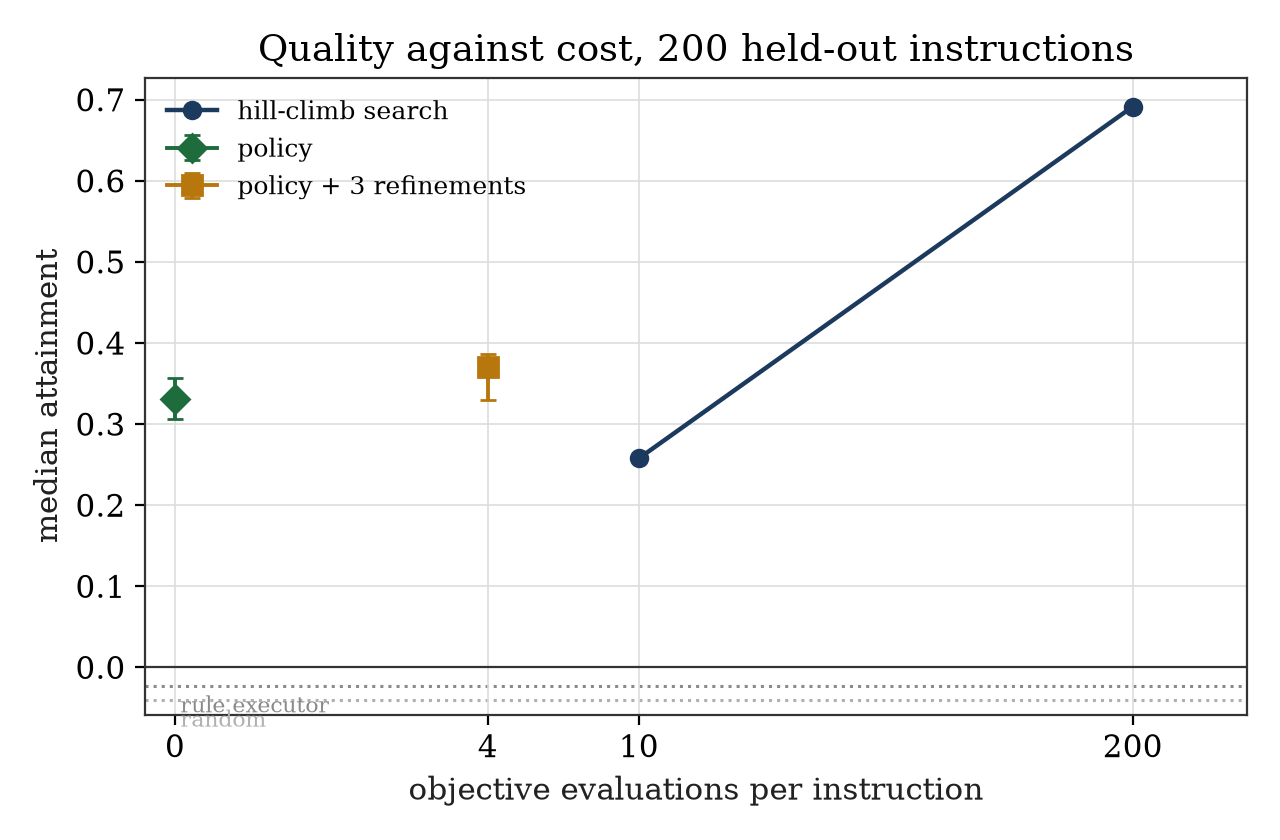
\includegraphics[width=\linewidth]{screenshots/results-frontier.png}
  \end{subfigure}\hfill
  \begin{subfigure}[t]{0.48\linewidth}
    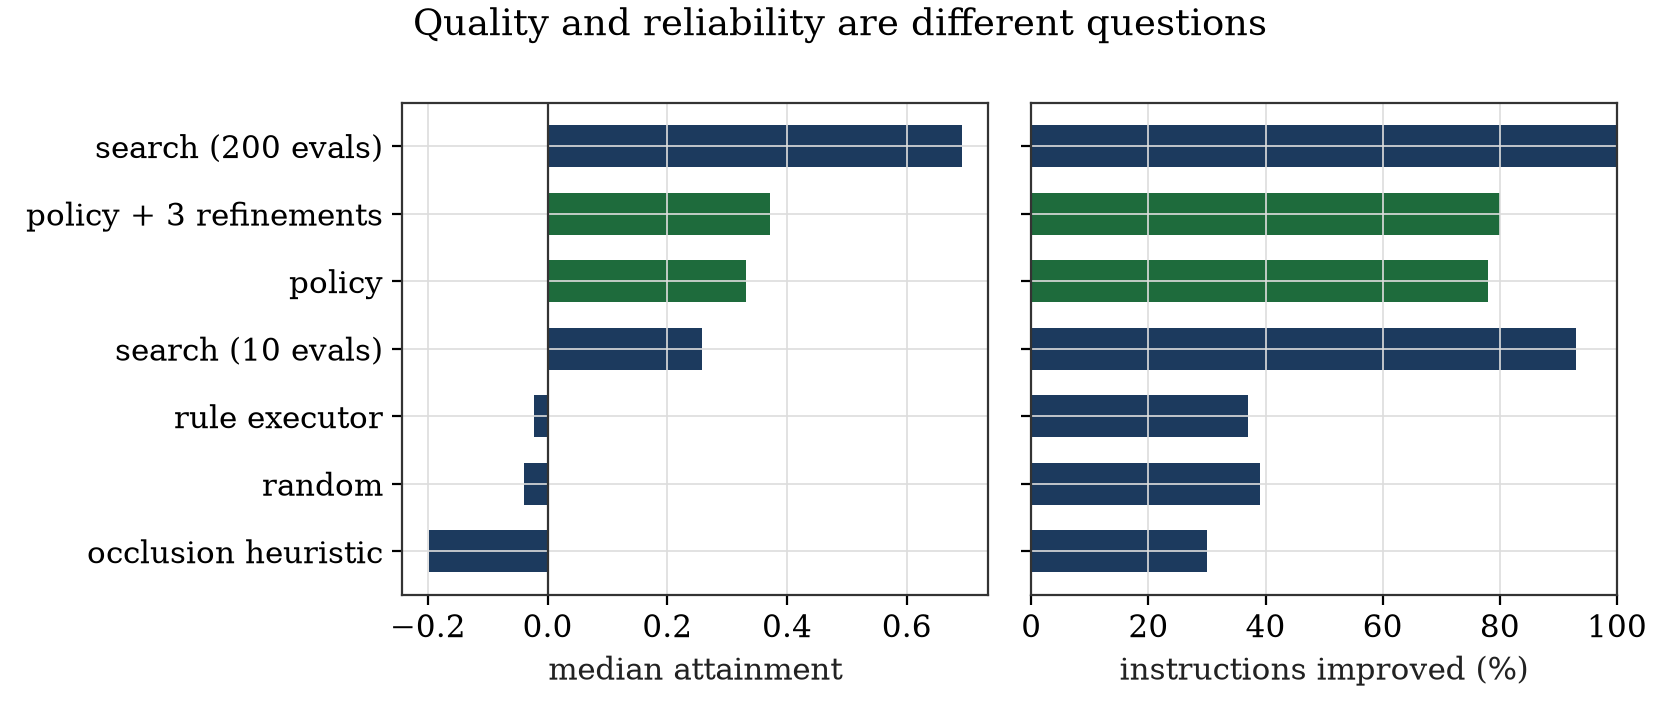
\includegraphics[width=\linewidth]{screenshots/results-reliability.png}
  \end{subfigure}
  \caption{Quality against cost, and quality against reliability --- the
  same table, plotted two ways. Generated by \code{plots.held\_out\_results}
  directly from the \code{rl.vis\_eval} result files; nothing in these
  figures recomputes a score.}
\end{figure}

\begin{figure}[h]
  \centering
  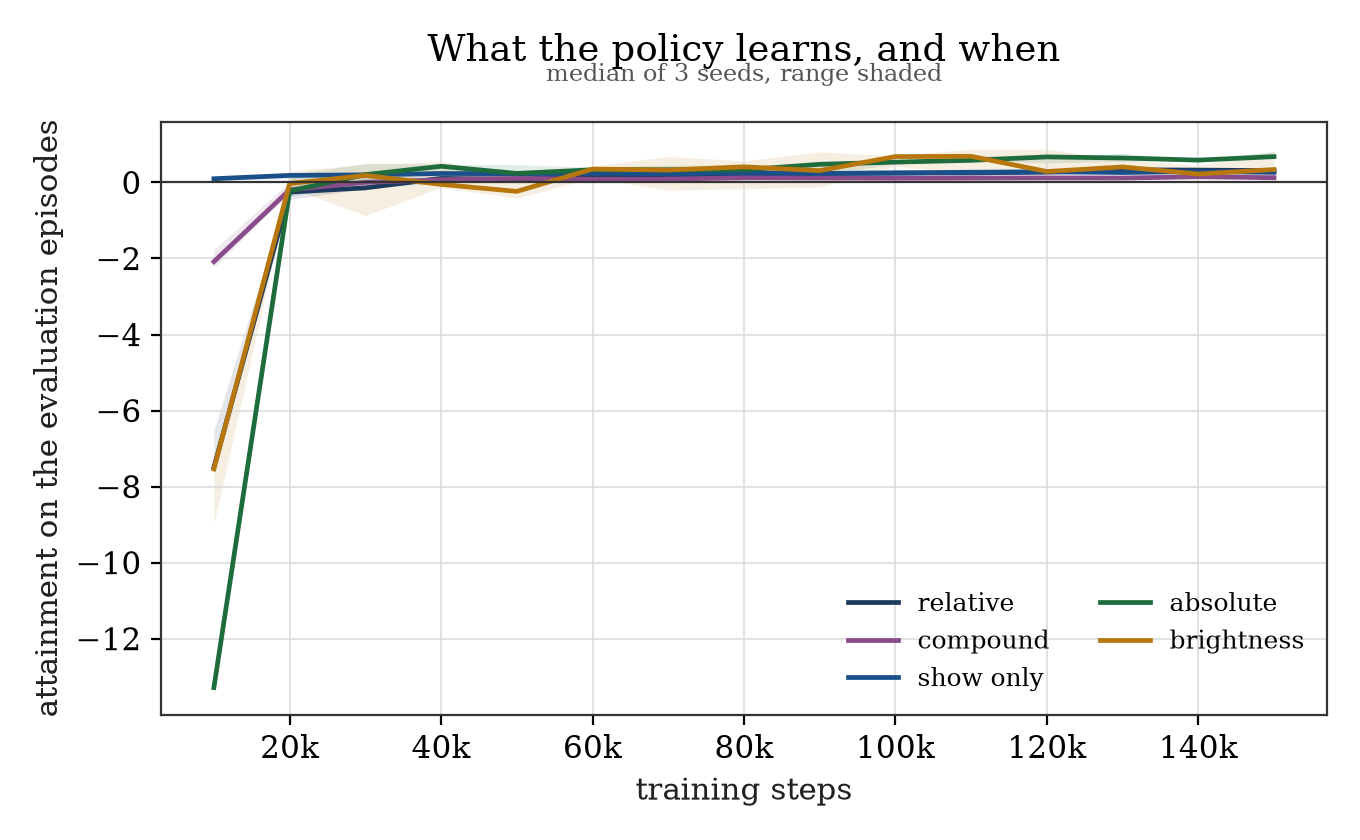
\includegraphics[width=0.78\linewidth]{screenshots/results-kind-curves.png}
  \caption{Attainment per instruction kind over training, median of the
  three v4 seeds, range shaded. Absolute, brightness and relative plateau
  comfortably positive; compound and show-only plateau near zero.}
\end{figure}

\begin{table}[h]
\centering\small
\begin{tabular}{@{}lc@{}}
\toprule
\textbf{Instruction kind} & \textbf{Median of medians, v4} \\
\midrule
absolute & $+0.511$ \\
brightness & $+0.561$ \\
relative & $+0.354$ \\
show only & $+0.166$ \\
compound & $+0.117$ \\
\bottomrule
\end{tabular}
\caption{Per-kind breakdown. Compound moved from the v3 figure of $+0.09$ to
$+0.117$ --- still weak, but not nothing.}
\end{table}

\subsection{Limitations, stated plainly}
\label{sec:limitations}

\begin{itemize}[itemsep=2pt, topsep=2pt]
\item \textbf{\code{show\_only} is not solved for the policy}
  (\cref{sec:v4-fix}) --- the reward no longer rewards the wrong thing, but
  nothing has yet taught the policy the right thing.
\item \textbf{\code{hill\_climb}'s coordinate descent finds the same
  ``suppress everything, light up unclassified tissue'' local optimum} on
  \code{show\_only}, from the default start and from randomised starts, even
  under the corrected objective. The fix removes the wrong incentive; it
  does not guarantee a greedy local search finds the right one. Left
  unaddressed deliberately --- changing search behaviour would need its own
  budget re-validation.
\item \textbf{Vessels answer on exactly one dataset} (\code{ts\_s1379}, \cref{sec:vessels-gate}).
\item \textbf{Out-of-source generalisation has never been formally
  evaluated}, despite \code{datasets.OUT\_OF\_SOURCE\_CT} and \code{rl.vis\_eval
  --split out\_of\_source} existing for exactly that.
\item \textbf{Compound instructions remain the second-clearest capability
  gap} ($+0.117$) after show-only.
\end{itemize}

\newpage
\section{The web application}

\subsection{Backend architecture}

\code{server.py} is a single FastAPI application plus one included router
(\code{collect.router}). All mutable state lives in one \code{Session}
object --- module-level, not per-request --- persisted to
\code{out/ui\_session.json} after every command so a server restart resumes
where the session left off. \code{Session.history} is an append-only list of
\emph{steps}; \code{cursor} is the current position, so back/forward are
just cursor moves, not re-computation.

\begin{table}[h]
\centering\small
\begin{tabular}{@{}lp{9.6cm}@{}}
\toprule
\textbf{Field} & \textbf{What it holds} \\
\midrule
\code{id}, \code{timestamp} & step identity \\
\code{cmd\_text}, \code{cmd\_dict} & what was said/typed, and its parsed form \\
\code{params} & the 24-float transfer function, after this step \\
\code{camera} & azimuth/elevation/zoom \\
\code{image\_b64}, \code{image\_path} & the rendered PNG, inline and on disk \\
\code{masses} & legacy opacity-mass readout over the retired HU bands \\
\code{class\_visibility} & per-goal-class visibility share --- the policy's own metric \\
\code{curve}, \code{histogram} & the transfer-function curve and volume histogram, added today (\cref{sec:tf-panel}) \\
\code{features} & coverage/brightness features straight off the rendered image \\
\code{mode} & ``exact'' \textbar\ ``search'' \textbar\ ``policy'' \textbar\ ``camera'' \\
\code{parser\_requested/used/fallback} & which parser was asked for vs.\ what actually ran \\
\bottomrule
\end{tabular}
\caption{Every field \code{server.\_render\_step} writes onto a step (\code{server.py}).}
\end{table}

\subsection{API reference}

\begin{table}[h]
\centering\small
\begin{tabular}{@{}lll@{}}
\toprule
\textbf{Route} & \textbf{Method} & \textbf{Purpose} \\
\midrule
\code{/} & GET & serves \code{static/index.html} \\
\code{/api/state} & GET & current step + cursor/total \\
\code{/api/back}, \code{/api/forward} & POST & move the history cursor \\
\code{/api/datasets} & GET & list loadable dataset names \\
\code{/api/datasets/\{name\}/metadata} & GET & dimensions/spacing for the local vtk.js viewer \\
\code{/api/datasets/\{name\}/chunks/\{i\}} & GET & chunked raw volume bytes for the local viewer \\
\code{/api/commands} & GET & the command reference (\code{COMMANDS.md}'s source) \\
\code{/api/dataset} & POST & switch the active dataset \\
\code{/api/command} & POST & parse + apply/search/answer one instruction \\
\code{/api/compare} & POST & answer one instruction four ways without advancing the session \\
\code{/api/compare/sweep} & POST & the same four ways, across many sampled instructions \\
\code{/api/scenes/transition} & POST & append a de-duplicated scene-transition record \\
\code{/api/transcribe} & POST & voice $\rightarrow$ text via faster-whisper \\
\code{/collect} & GET & the blind preference-collection page \\
\code{/api/collect/next} & POST & the next pair to judge \\
\code{/api/collect/judge} & POST & record a judgment \\
\bottomrule
\end{tabular}
\caption{The complete route table, \code{server.py} + \code{collect.py}.}
\end{table}

\code{/api/command} and \code{/api/compare} both accept a \code{parser}
field (default \code{"llm"}) and a \code{mode} field (\code{"exact"}
\textbar\ \code{"search"} \textbar\ \code{"policy"}). \code{/api/compare}
parses the instruction \emph{once} and builds one goal from it, so all four
arms answer the identical parsed command --- a bad parse then makes every arm
wrong together, read as a parsing problem rather than a policy problem, not
four independently-wrong answers.

\subsection{Frontend}

\begin{figure}[h]
  \centering
  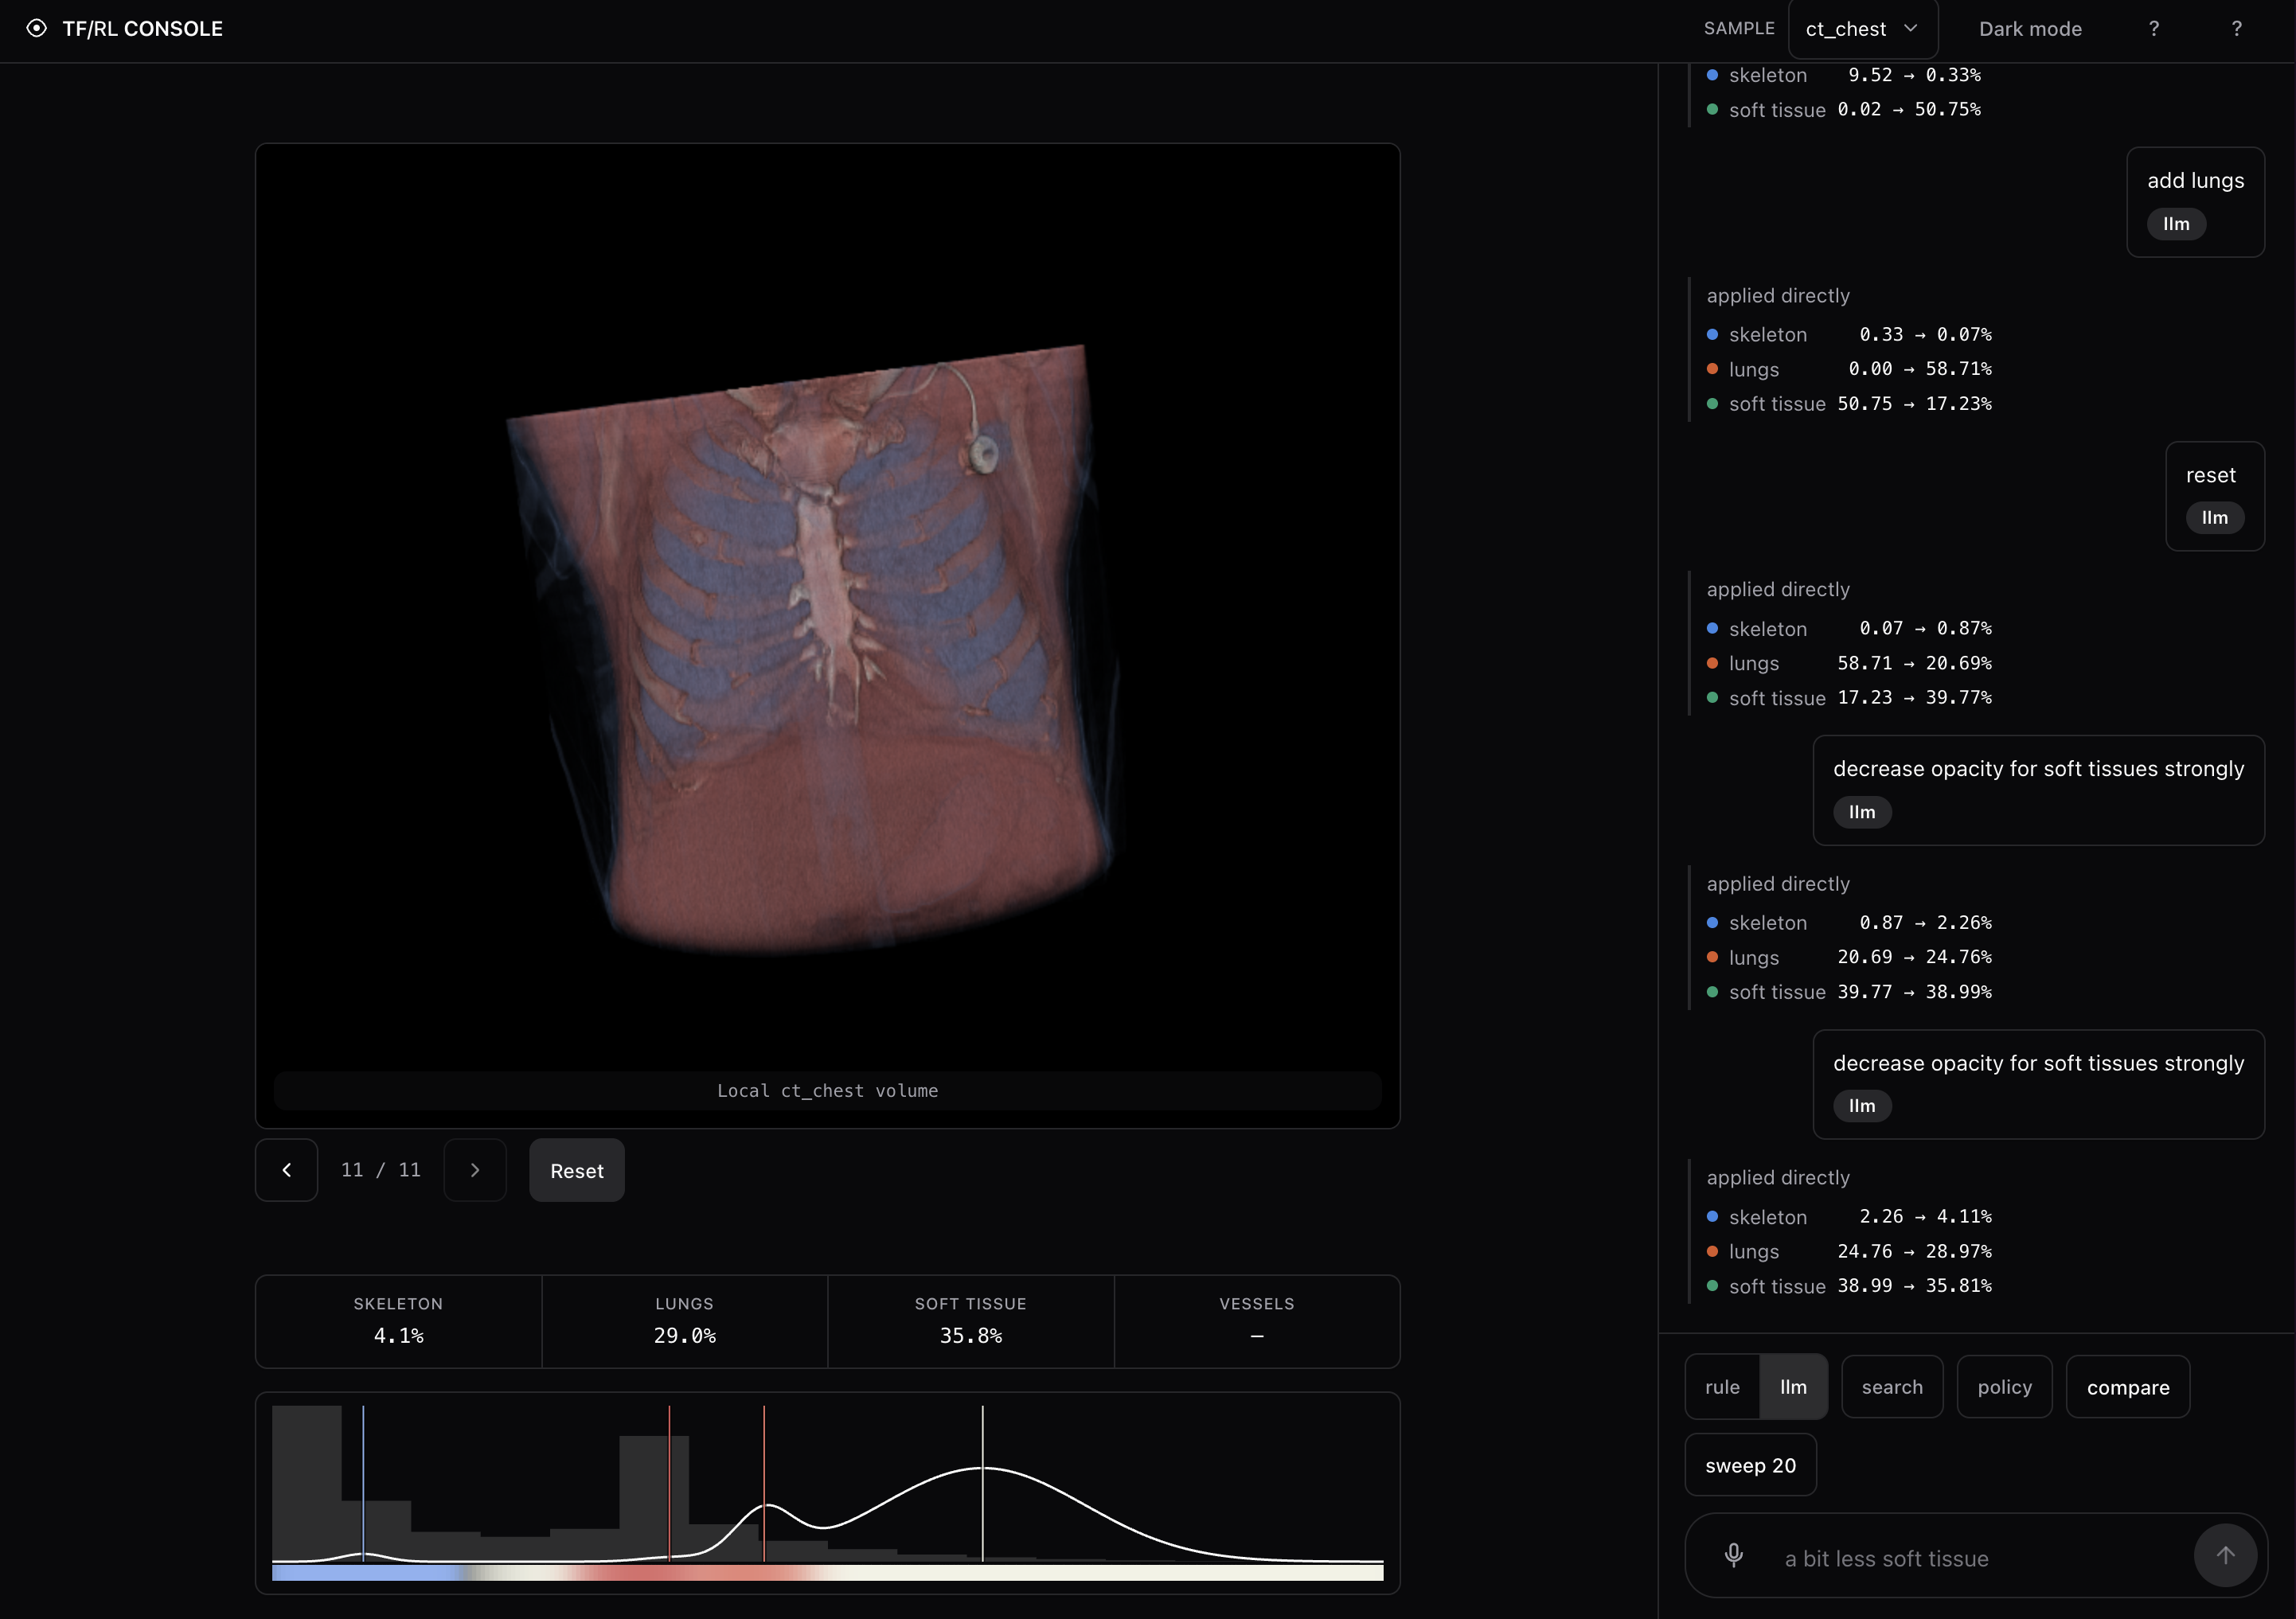
\includegraphics[width=0.92\linewidth]{screenshots/ui.png}
  \caption{The viewer mid-session: a render, the instruction history with
  each command's per-class visibility delta, and the histogram/transfer-function
  curve panel (\cref{sec:tf-panel}) at the bottom.}
\end{figure}

\code{static/index.html} is a single page: a top bar (dataset picker, theme
toggle, help), the viewer region (render, camera nav, per-class telemetry
tiles, the curve panel), and a chat-style console (message history, a
toolbar of mode toggles, and a text/voice composer). No build step --- plain
HTML, CSS, and vanilla JavaScript, styled with a shadcn-inspired zinc theme
implemented as CSS custom properties rather than an actual shadcn/React
component library (a deliberate constraint from this UI's own design spec).

\code{static/app.js} owns all application state and API calls. Every
state-changing action funnels through \code{refresh(data)}, which updates
the rendered image, the telemetry tiles, and (as of today) the curve panel
--- one place that stays in sync whenever a new step arrives, regardless of
which action produced it. \code{static/viewer.js} wraps \code{vtk.js}: it
streams a dataset in chunks (\code{/api/datasets/\{name\}/chunks/\{i\}}),
reconstructs a Fortran-ordered \code{Float32Array}, and applies
transfer-function and camera changes locally in the browser without a
server round trip for every render.

\subsection{The histogram/transfer-function curve panel}
\label{sec:tf-panel}

Added this session, directly answering the original project brief's request
for ``a visual guide that plots the current transfer function on top of the
histogram.'' Computed entirely server-side and attached to every step:

\begin{itemize}[itemsep=2pt, topsep=2pt]
\item \code{curve}: \code{transfer.\_opacity\_and\_color\_at} sampled at the
  same 256 points \code{visibility.py}'s own lookup table uses
  (\code{visibility.lut\_values()}) --- a pure function of that step's
  \code{params}, so it's available even for a dataset with no visibility model.
\item \code{histogram}: the loaded volume's own intensity histogram --- the
  \emph{same} 16-bin histogram \code{rl.oneshot\_env}'s observation already
  carries, so the chart shows exactly what the policy sees, not a separate
  visualisation-only computation.
\end{itemize}

The frontend (\code{drawTfCurve} in \code{app.js}) draws the histogram
sqrt-scaled (a raw CT histogram is dominated by one huge air/background bin
that would otherwise flatten every tissue peak to invisible), the opacity
curve traced over it, a colour ramp along the bottom built from the same RGB
samples, and tick marks at the four anatomical peak centres in each peak's
\emph{actual} transfer-function colour (\code{transfer.ANATOMICAL\_COLOURS})
--- not the telemetry tiles' own accent hues, which are a UI-only palette
and would otherwise contradict the ramp directly beneath them.

\subsection{Voice}

\code{asr.py} wraps \code{faster-whisper}; the mic button holds to record
(push to talk, or Space), \code{/api/transcribe} returns text, and that text
enters the exact same \code{/api/command} path a typed instruction would.
There is no separate ``voice mode'' in the backend --- voice is a text
source, nothing more.

\newpage
\section{Preference collection and RLHF}
\label{sec:preferences}

The eventual reward-model stage this system is built towards: \code{/collect}
shows one instruction and two candidate results (six views each), blind ---
no indication of which arm produced which. A rater presses A, B, equal, or
skip. Roughly one item in five is drawn from a fixed anchor pool
(\code{rl.candidates.anchor\_items}) --- the same items, same order, for
every rater --- so cross-rater agreement is measurable; the rest are sampled
fresh. Roughly one item in ten silently repeats an earlier one with sides
swapped, measuring a single rater's own self-consistency, the ceiling any
reward model trained on their judgments can reach.

\begin{lstlisting}
python -m tools.merge_preferences out/*.jsonl --out out/preferences_merged.jsonl
\end{lstlisting}

merges multiple raters' files (de-duplicated on pair + rater, latest
timestamp wins) and reports raw agreement plus linearly-weighted Cohen's
kappa per rater pair on shared anchor items, and Krippendorff's alpha across
all raters together.

\status{0 clean preference judgments exist. 54 were collected before the
colour-decode bug (\cref{sec:evolution}) was fixed and are archived, not
used, because a rater could tell the policy's renders apart by their
greyness alone --- not a blind comparison. Reward-model training and RLHF
have not started.}

\newpage
\section{Setup and reproduction}

\begin{lstlisting}
python3 -m venv .venv && source .venv/bin/activate
python -m pip install --upgrade pip
python -m pip install -r requirements.txt
python -m pytest -q -m "not slow"    # fast suite, 678 passing as of today
python -m pytest -q                  # everything
python server.py                     # http://127.0.0.1:8000
\end{lstlisting}

Run everything from the repository root --- the code uses relative paths
such as \code{out/} and \code{static/}. LLM parsing needs Ollama running
locally (\code{ollama serve \&\& ollama pull qwen2.5:7b}); without it, every
LLM request falls back to the rule parser automatically. First voice use
downloads and caches a Whisper model. \code{docs/REPRODUCE.md} has every
command from raw data to the held-out table with real timings.

\section*{Reading further}

\begin{itemize}[itemsep=2pt, topsep=2pt]
\item \code{docs/rl-paper.typ} --- the thesis argument: problem, method,
  results, and the measurement incidents, written to be read start to end.
\item \code{docs/STATUS.md} --- the living ``where things stand'' document,
  dated, rewritten whenever something material changes.
\item \code{docs/REPRODUCE.md} --- every command from raw data to the held-out table.
\item \code{README.md} --- the short version, for anyone who wants the claim
  and a demo in two minutes.
\item \code{COMMANDS.md} --- the full instruction grammar, generated from
  \code{commands.COMMAND\_REFERENCE} (\code{python -m tools.gen\_commands\_doc}).
\end{itemize}

\end{document}
